\section{Siamese networks}
\label{siamese networks}

Section~\ref{acrhitecture} describes our overall network architecture for entity matching. Section~\ref{loss_functions} enumerates the different loss functions which have been used in prior work, and a new loss function which appears to do better in metric learning for entities.  Section~\ref{triplet_selection} describes a novel triplet selection mechanisms for entity matching.

\subsection{Network Architecture}
\label{architecture}
\begin{figure}
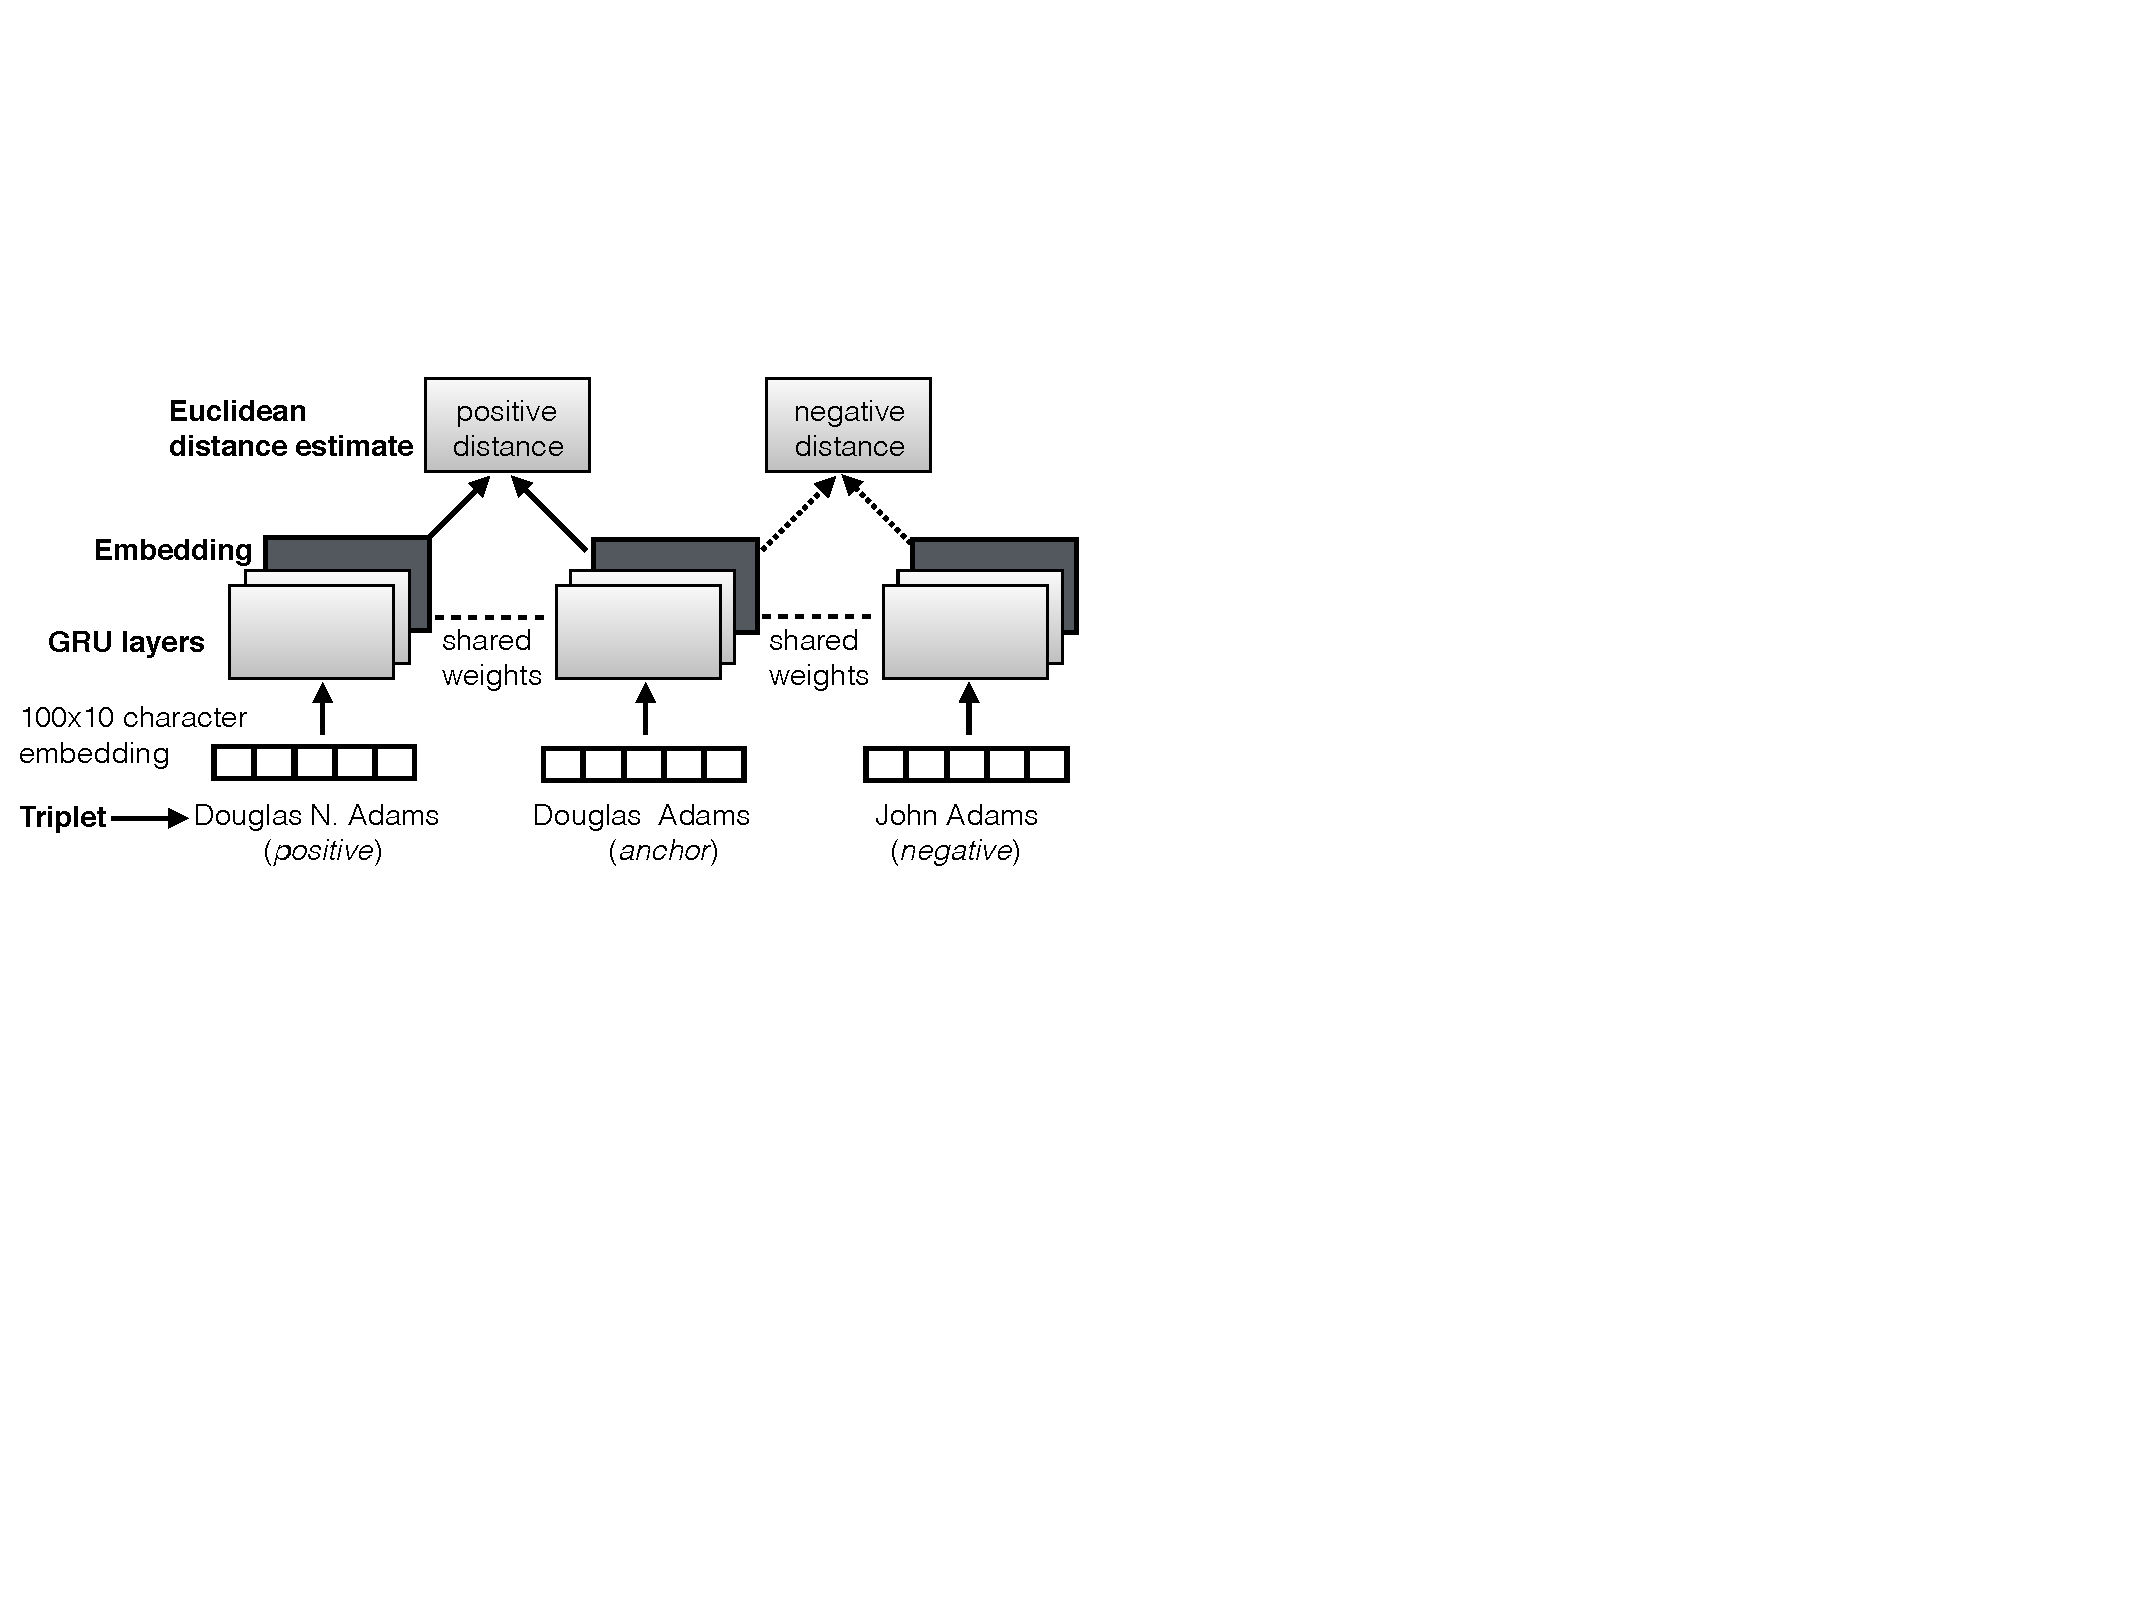
\includegraphics[width=1.0\linewidth]{triplet_siamese_network}
\caption{Architecture of the siamese network}
\label{siamese_nets}
\end{figure}

Figure~\ref{siamese_nets} illustrates overall network architecture we used to build a system for fuzzy joins.  Input vectors were computed assuming a maximum name length of 10 for each entity (i.e., no entity could have a name that spanned more than 10 words).  A 100 dimensional character embedding was computed for each `word' in the entity using pretrained embeddings \cite{hashimoto-jmt:2017:EMNLP2017}, which resulted in a 100 x 10 character encoding for each name used in a triplet.  As described earlier, in a triplet, each entity name (or \textit{anchor}) is paired with another name for the same entity (or \textit{positive}), and with a name for a completely different entity (or \textit{negative}).  The three input vectors from each triplet are fed to three identical networks that share the same weights.  Weight sharing ensures that the networks learn the same mapping function for any given input vector.  In our implementation, each of the three networks had 4 stacked layers of 128 unit Gated Recurrent Units (or GRUs) to capture the sequential nature of the input.  

GRUs are a type of recurrent network \cite{cho-al-emnlp14} where each hidden unit updates its weights at a specific step in the sequence $t$ based on the current input $x_t$ and the value of the hidden unit from the prior step $h_{t-1}$.  $r_t$ is a reset gate which determines whether the state from the previous step $h_{t-1}$ should be ignored. $z_t$ is an update gate which determines whether the current hidden state should be updated with the new hidden state $\tilde{h_t}$.  Equations~\ref{eq_1}-\ref{eq_4} that govern the update at $h_t$, as summarized by \cite{colah}.
\begin{equation}
z_t = \sigma(W_z . [h_{t-1}, x_t])
\label{eq_1}
\end{equation}

\begin{equation}
r_t = \sigma(W_r . [h_{t-1}, x_t])
\label{eq_2}
\end{equation}

\begin{equation}
\tilde{h_t} = tanh (W . [r_t * h_{t-1}, x_t])
\label{eq_3}
\end{equation}

\begin{equation}
h_t = (1- z_t) * h_{t-1} + z_t * \tilde{h_t}
\label{eq_4}
\end{equation}

The output of the last layer shown in the Figure~\ref{siamese_nets} as a dark gray layer produces a vector embedding for the inputs.  These are fed to two layers which compute a euclidean distance between the \textit{anchor} and the \textit{positive} elements of a triplet (\textit{positive distance}), and the \textit{anchor} and the \textit{negative} elements of a triplet (\textit{negative distance}).  Conceptually, there are two objectives in metric learning, one to minimize \textit{positive distances}, and the other to maximize \textit{negative distances}.  As described below, this dual objective is achieved by different loss functions in the literature.

\subsection{Loss functions}
\label{loss_functions}
Let $\mathbf{x}$ represent an embedding for an entity name, and $\bf{x_{a}}$, $\bf{x_{p}}$, $\bf{x_{n}}$ reflect the vector embeddings of the \textit{anchor}, \textit{positive} and \textit{negative}, respectively.  We investigated four different loss functions to explore their effectiveness for the entity metric learning problem.
\subsubsection{Triplet loss}

\begin{figure}
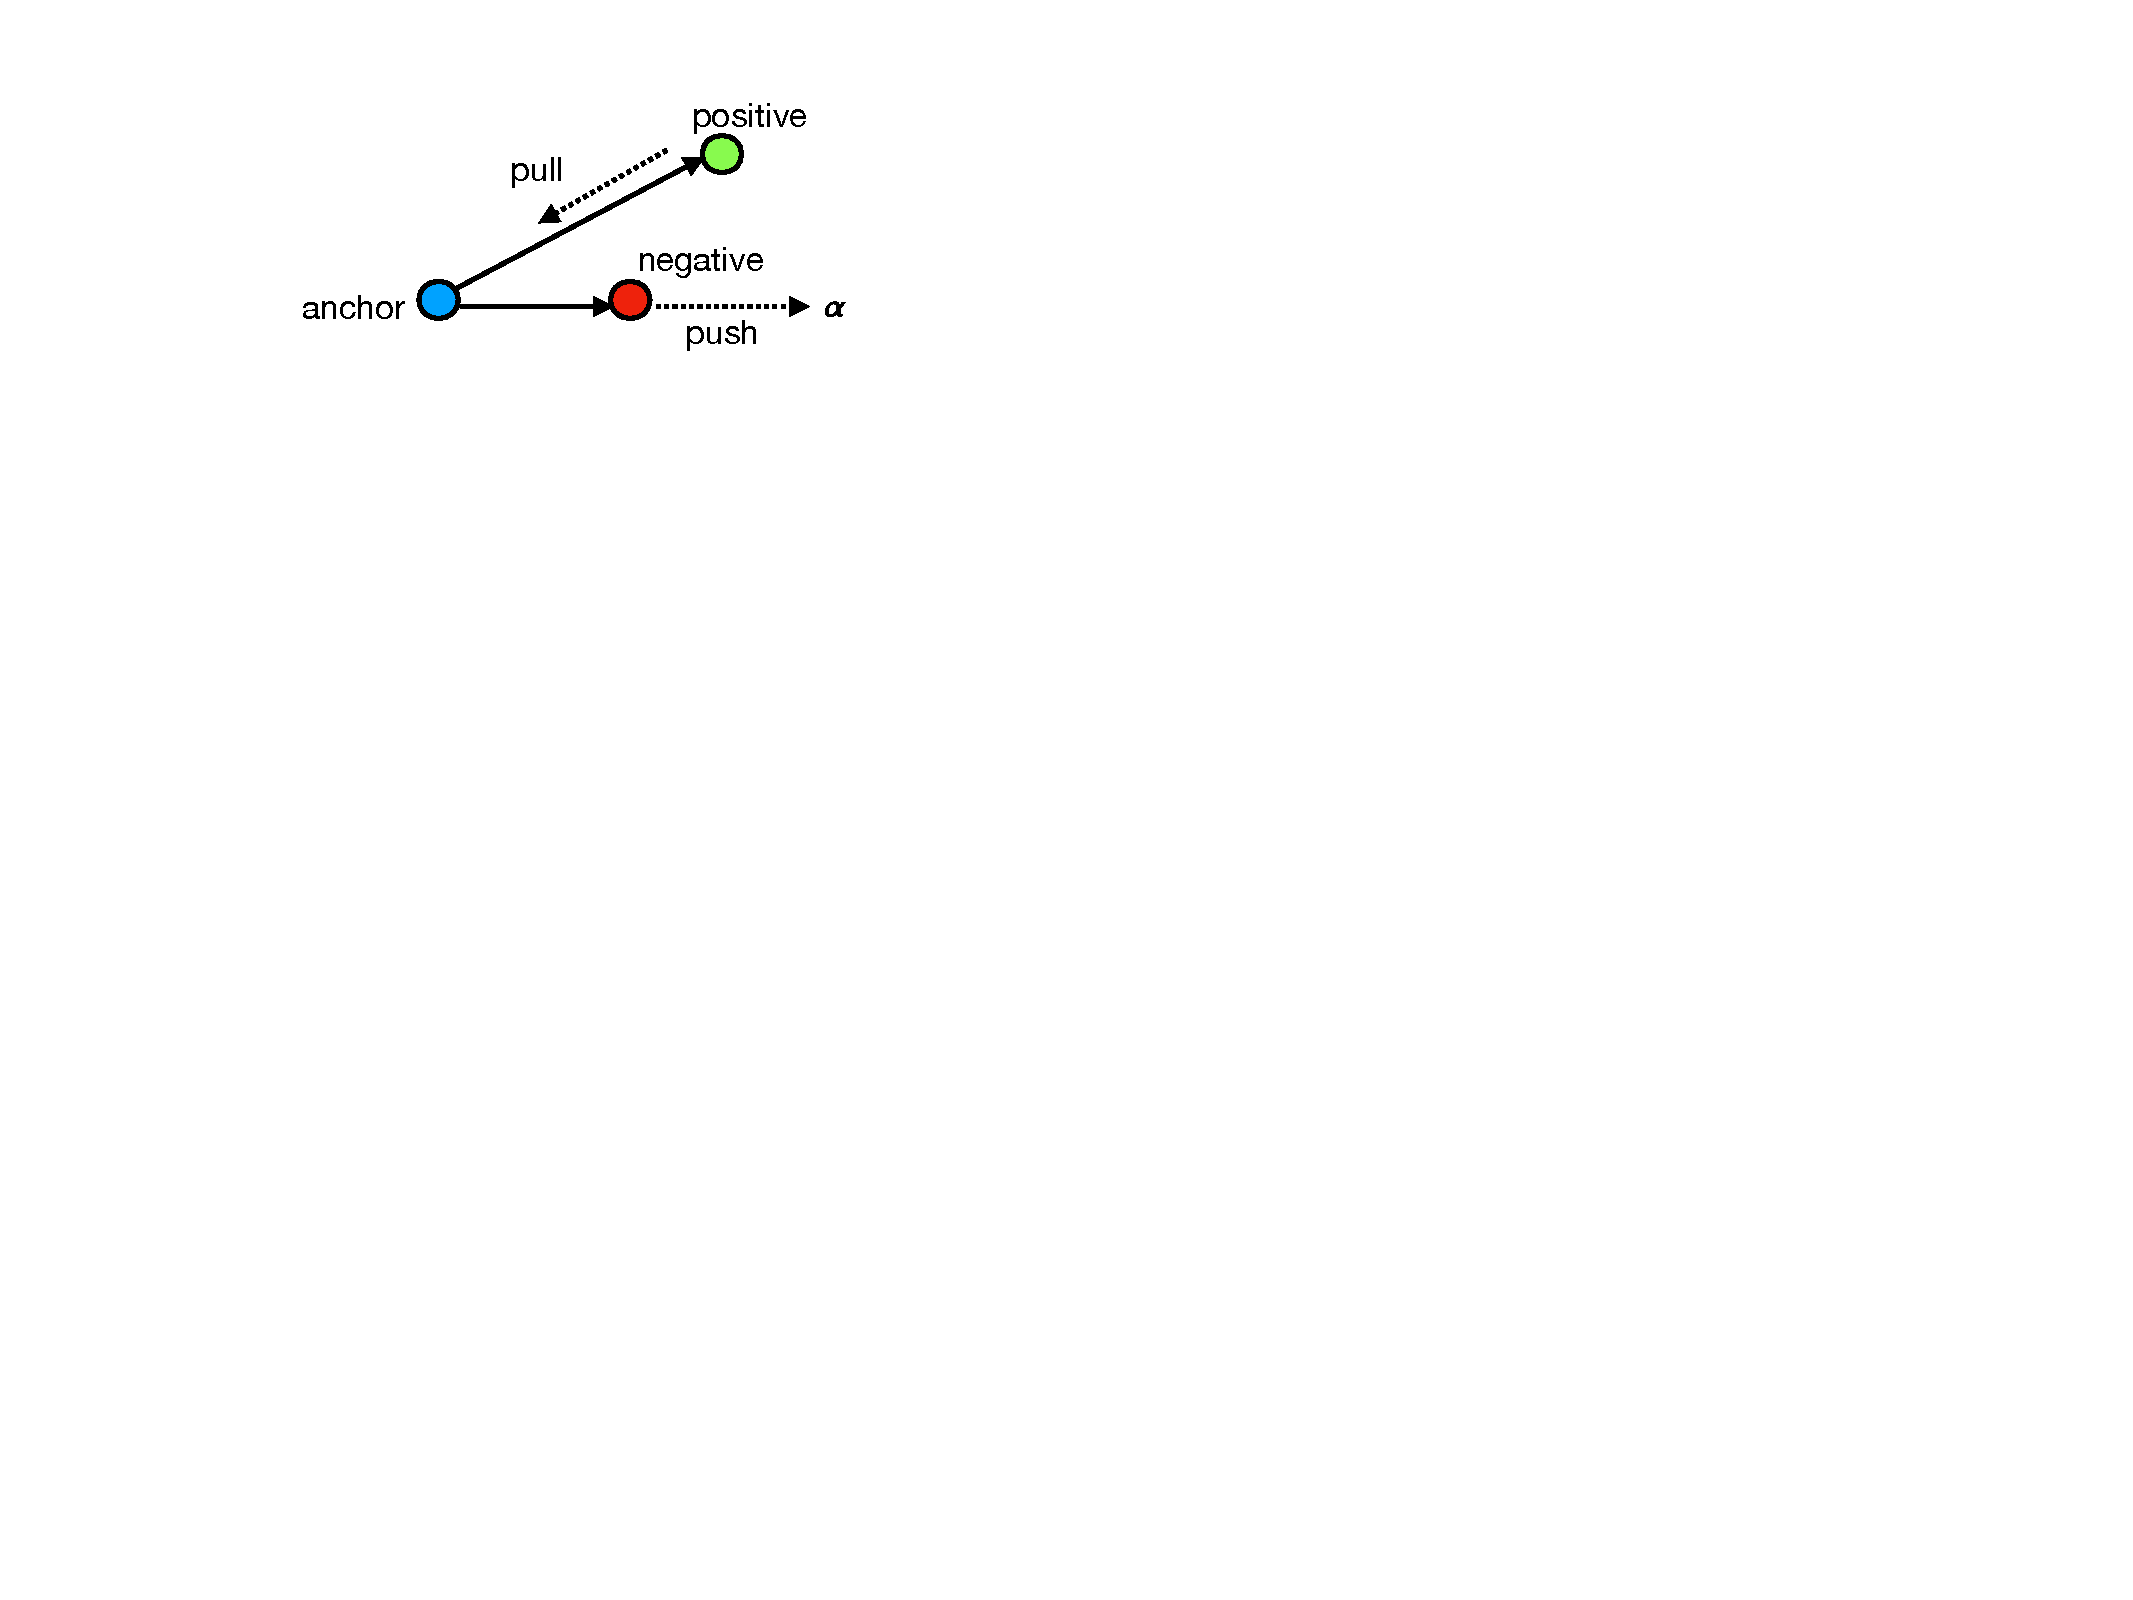
\includegraphics[width=0.5\linewidth]{schroff_triplet}
\caption{Triplet loss}
\label{schroff_loss}
\end{figure}

For face recognition, Schroff et al. \cite{DBLP:conf/cvpr/SchroffKP15} propose a triplet loss function where the \textit{positive distances} for each triplet $i$ in the set of $N$ triplets is separated from \textit{negative distances} by a margin of $\alpha$, as shown in Figure~\ref{schroff_loss}.  For each of $N$ triples, $l_{triple}$ reflects the loss for a given triple as follows:
\begin{equation}
  l_{triple} =  \left[\|\bf{x_a} - \bf{x_p}\|^2 - \|\bf{x_a} -\bf{x_n}\|^2 + \alpha \right]_+
\label{schroff}
\end{equation}
where
\begin{equation}
 \left[.\right]_{+} = max(0, .)
\end{equation}
and the loss function that is minimized across all $N$ triples is given by
\begin{equation}
 L = \sum_{i}^{N} l_{triple}
\end{equation}
Note that in this formulation, it is assumed that embedding is normalized so $\|\bf{x} \| = 1$ because this normalization is robust across variations in illumination and contrast.  The value of $\alpha$ in the original work is a hyper-parameter that \cite{DBLP:conf/cvpr/SchroffKP15} was set to 0.2.

\subsubsection{Improved Loss}

\begin{figure}
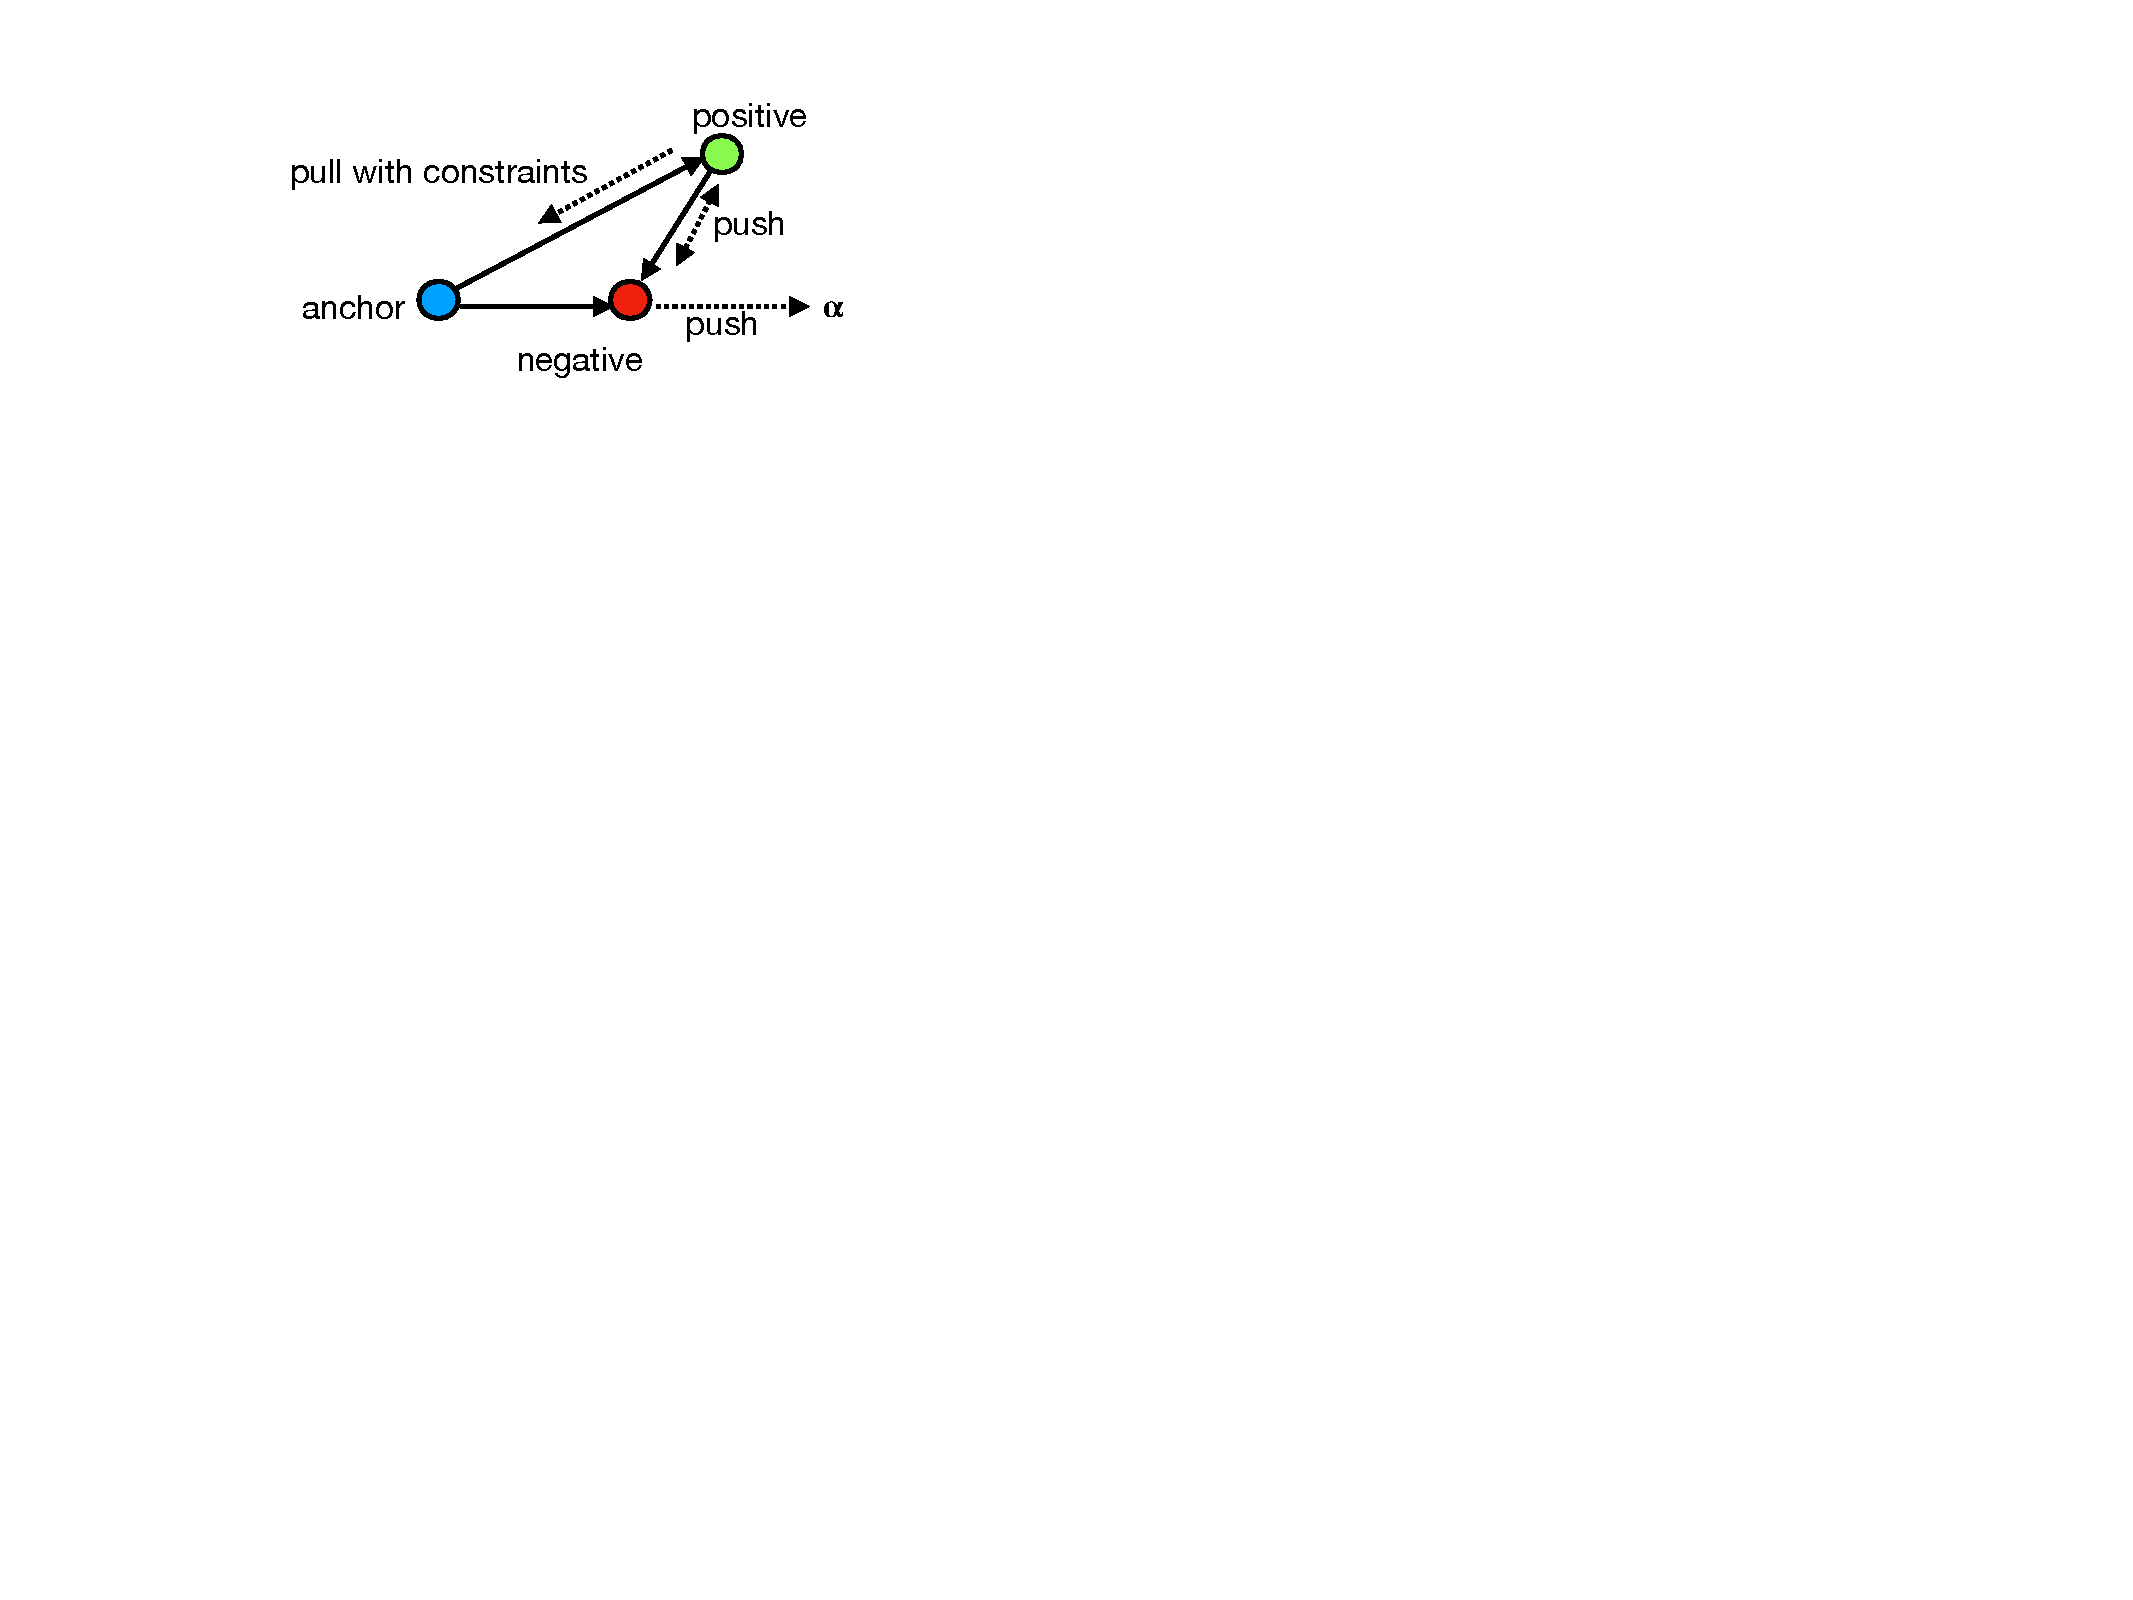
\includegraphics[width=0.5\linewidth]{modified_loss}
\caption{Modified loss}
\label{modified_loss}
\end{figure}

 An improvement over the triplet loss function is proposed by \cite{DBLP:conf/cvpr/SchroffKP15} for the recognition of faces in videos \cite{Zhang:2016:DML:3088616.3088665}.  Conceptually, this function that we refer to as `improved loss' in the paper considers the distances from the \textit{positive} element of the triplet to the \textit{negative} element as well, and tries to maximize that difference as well as the distance from \textit{anchor} to the \textit{negative}.  In addition,it corrects the fact the  original triplet loss function has no constraints on how close the positive distance should be.  For instance, it is possible for the \textit{anchor} and \textit{positive} form a large cluster with a large intra-class distance. The equations that achieve these constraints are described below.  Equation~\ref{psi} tries to reduce intra-class distance by ensuring it is less than $\hat{\alpha}$.  Equation~\ref{phi} tries to maximize inter-class distance by ensuring that the distance from the \textit{anchor} and \textit{positive} to the negative are both taken into account.  Equation~\ref{improved_loss} balances inter-class constraints with intra-class constraints with the parameter $\lambda$. 

\begin{equation}
  \psi_{triple} = \|\bf{x_{a}} - \bf{x_{p}}\|^2 - \hat{\alpha}
\label{psi}
\end{equation}
\begin{equation}
  \phi_{triple} = \|\bf{x_{a}} - \bf{x_{p}}\|^2 - (\|\bf{x_{a}}- \bf{x_{n}}\|^2 + \|\bf{x_{p}} - \bf{x_{n}}\|^2) / 2  + \alpha
\label{phi}
\end{equation}
\begin{equation}
  l_{triple} = max(0, \phi) + \lambda * max(0, \psi)
\label{improved_loss}
\end{equation}
The parameter $\hat{\alpha}$ for equation~\ref{psi} is set to 0.1, and $\lambda$ is set to .02 in equation~\ref{improved_loss}, and $\alpha$ was set to 1 in the paper \cite{Zhang:2016:DML:3088616.3088665}.  As in Schroff et al. \cite{DBLP:conf/cvpr/SchroffKP15}, the embeddings are normalized to 1.

\subsubsection{Angular Loss}

\begin{figure}
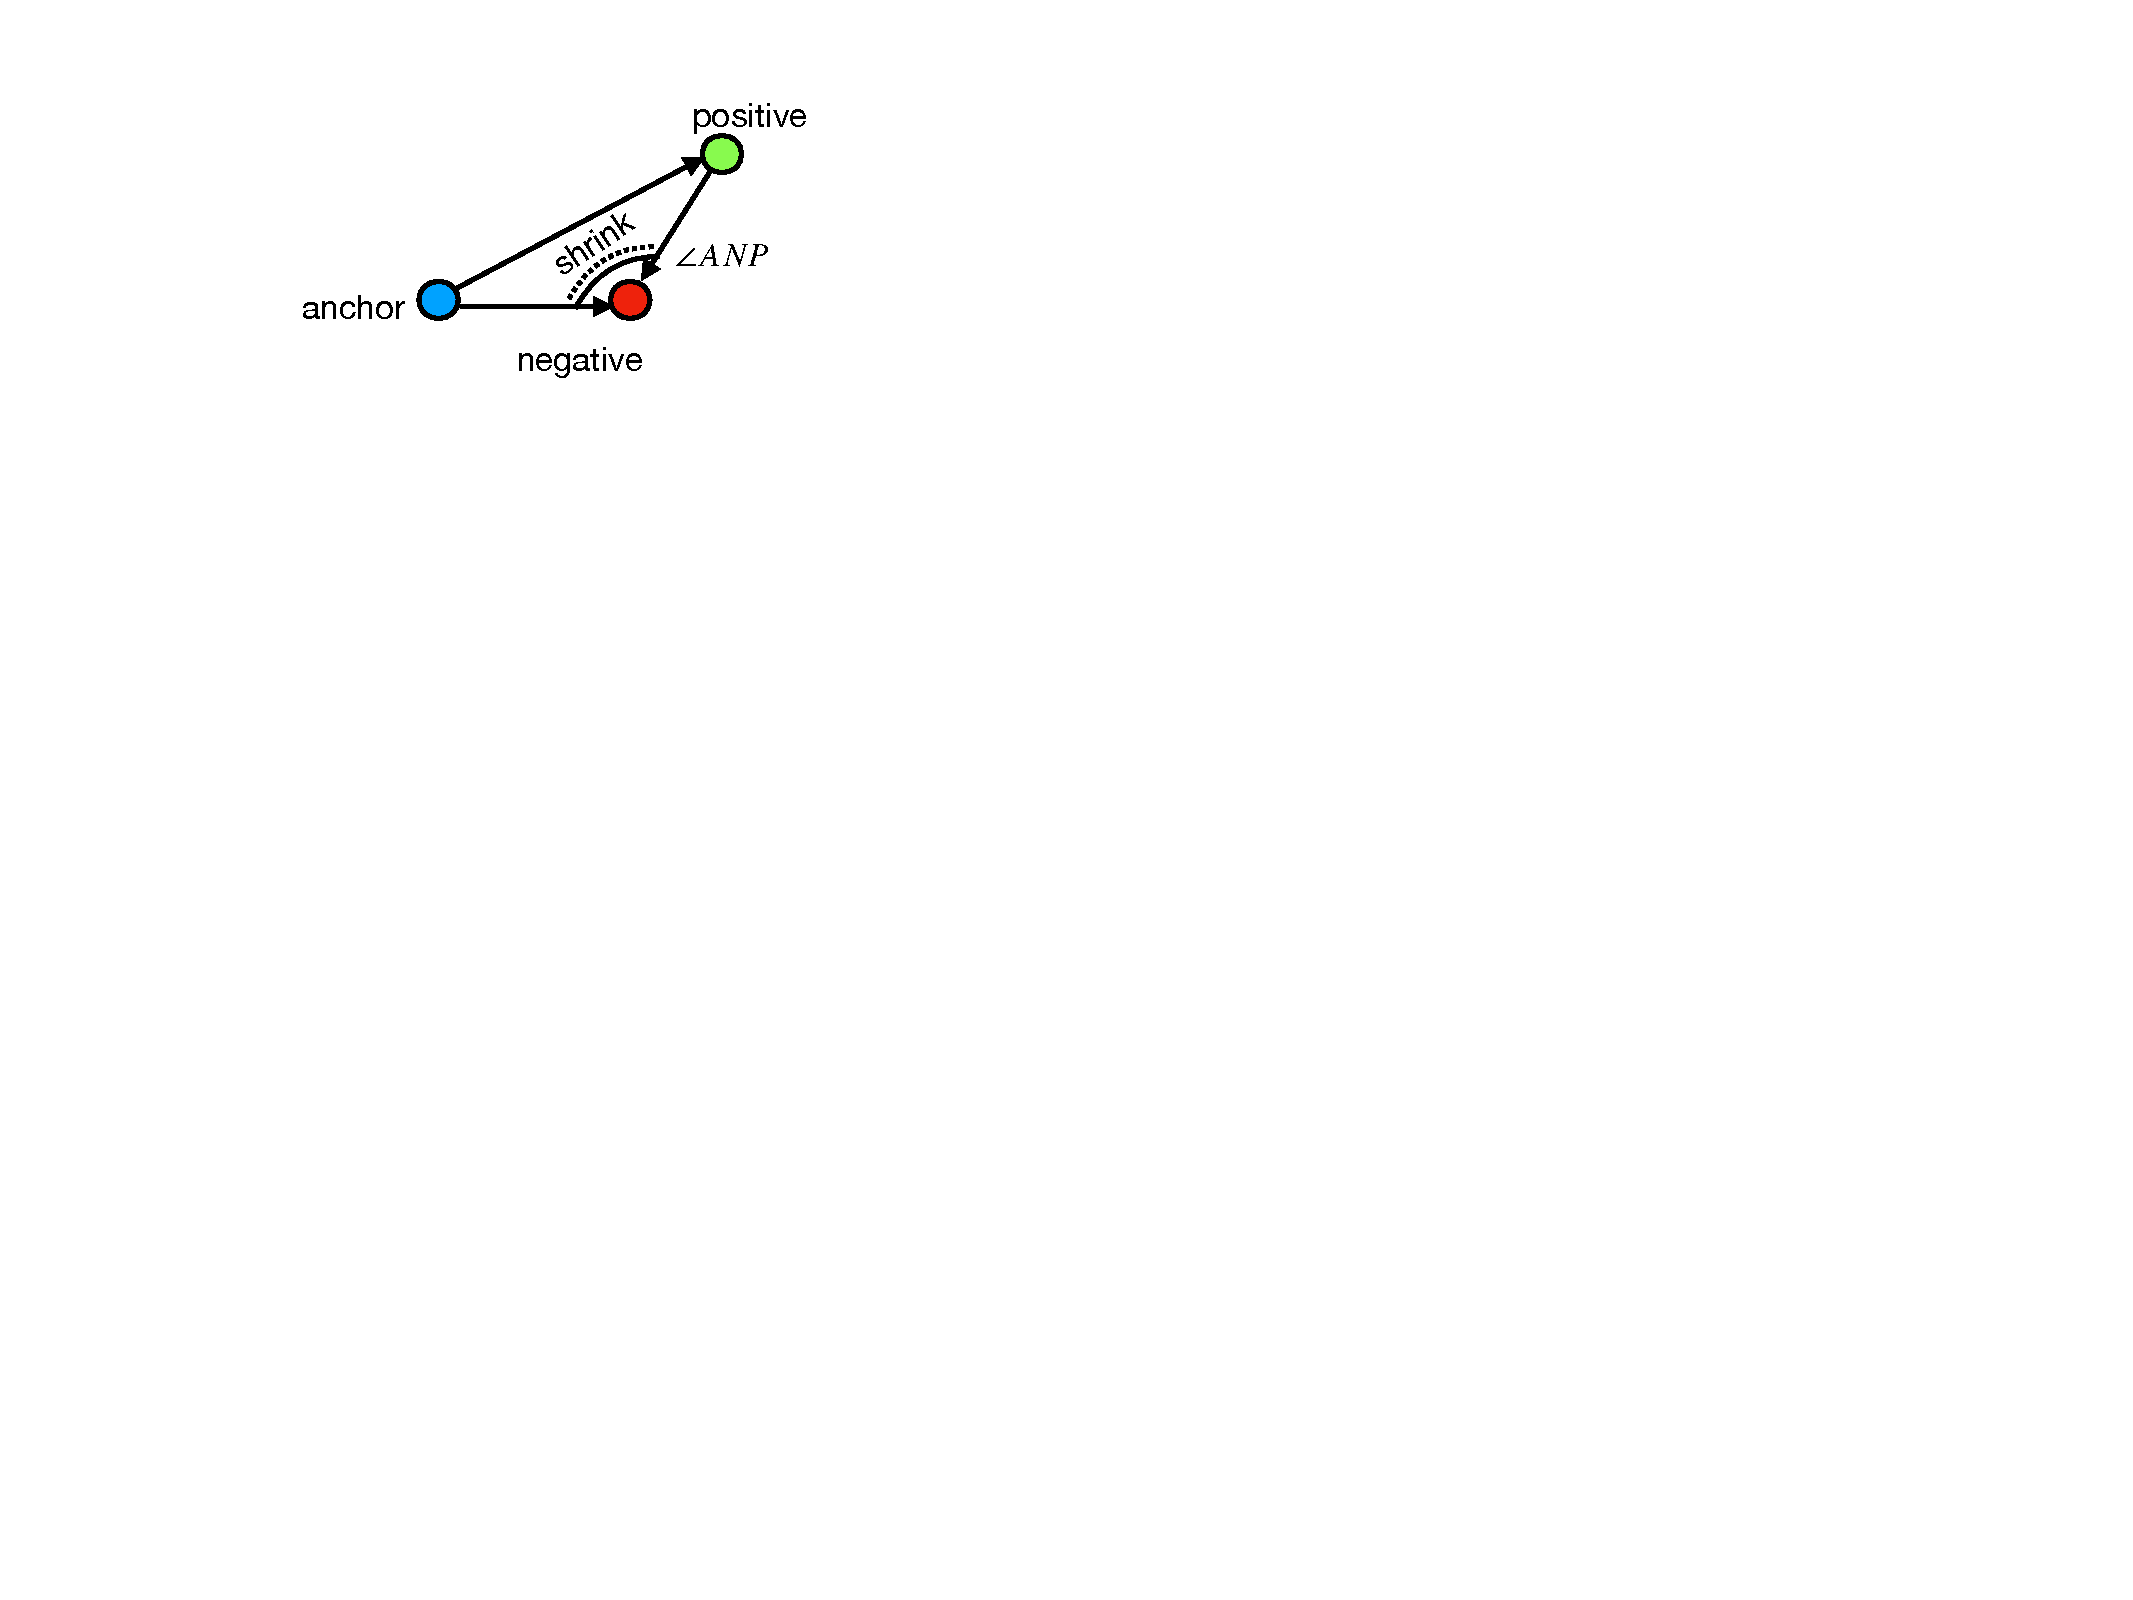
\includegraphics[width=1\linewidth]{angular_loss}
\caption{Angular loss}
\label{angular_loss}
\end{figure}

Wang et al. \cite{DBLP:journals/corr/abs-1708-01682} define a novel angular loss function which is not based on pairwise distances, but rather is based on the angles of the triangle formed by the \textit{anchor}, \textit{positive} and the \textit{negative} triplet.  Conceptually, they point out that since the \textit{anchor} and the \textit{positive} pairs belong to the same class, the angle formed by the \textit{anchor}, \textit{negative}, and \textit{positive} elements should be as small as possible within that triangle.  Their loss function is an attempt to minimize this angle, as defined in the equation below.
\begin{equation}
\bf{x_{c}} = (\bf{x_{a}} + \bf{x_{c}}) / 2
\end{equation}
\begin{equation}
l_{triplet} = \left[[\bf{x_{a}} - \bf{x_{p}}\|^2 - 4 \tan^2 \alpha \|\bf{x_{n}} - \bf{x_{c}}\|^2 \right])_{+}
\end{equation}
